\documentclass[11pt]{article}
\usepackage{amsmath, amssymb}
\usepackage{listings}
%\usepackage{mathtools}
\usepackage[utf8]{inputenc} % Swedish
\usepackage{xcolor}
\usepackage{graphicx}  % For figures
\usepackage{caption}
\usepackage{url}
\usepackage{mathtools} % mathclap

\usepackage{footnote}
\makesavenoteenv{tabular}
\makesavenoteenv{table}

\usepackage{array}
\newcolumntype{L}[1]{>{\raggedright\let\newline\\\arraybackslash\hspace{0pt}}p{#1}}
\newcolumntype{C}[1]{>{\centering\let\newline\\\arraybackslash\hspace{0pt}}p{#1}}
\newcolumntype{R}[1]{>{\raggedleft\let\newline\\\arraybackslash\hspace{0pt}}p{#1}}

\lstset{basicstyle=\ttfamily\footnotesize,breaklines=true}
\DeclareCaptionFont{white}{\color{white}}
\DeclareCaptionFormat{listing}{%
	\parbox{\textwidth}{\colorbox{gray}{\parbox{\textwidth}{#1#2#3}}\vskip-4pt}}
\captionsetup[lstlisting]{format=listing,labelfont=white,textfont=white}
\lstset{frame=lrb,xleftmargin=\fboxsep,xrightmargin=-\fboxsep}


\title{Learning Simulator \\ User's Guide}
\author{Markus Jonsson}
\begin{document}
\maketitle

\section{Installation instructions}

\section{How to run the program}
Use the control command \verb|lesim| to run Learning Simulator. Below are the available options.

\begin{lstlisting}[caption={\texttt{lesim} syntax}]
python lesim.py
Short for "python lesim.py gui"
    
python lesim.py gui
Start the Learning Simulator gui
    
python lesim.py run file1 [file2, file3, ...]
Run the script files file1, file2, ...
    
python lesim.py help
Display this help and exit
\end{lstlisting}

\section{Learning models}
This section will introduce the learning models that can be simulated in the program.
\begin{figure}[ht]
	\setlength{\unitlength}{1cm}
	\centering
	\begin{picture}(4,4)
	% l b r t
	% \put(0,0){\line(1,0){4}}
	% \put(0,0){\line(0,1){4}}	
	%
	% In MATLAB, run "figure,unifpartsim_subplot", then export pdf with width 15 cm.
	\put(0,0){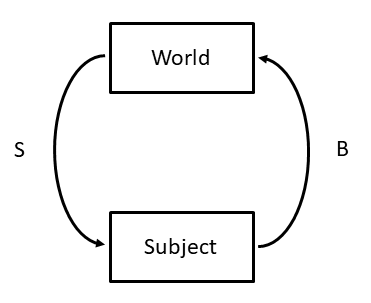
\includegraphics[scale=0.5,clip=true,trim=0 0 0 0]{Snurran.png}}
	\end{picture}	
	\caption{The world and the subject. \label{fig:snurran}}
\end{figure}
Figure~\ref{fig:snurran} illustrates the system we want to study.
The \emph{organism} has an output function that generates behavior and state transition functions
that update memories and other internal states.
The world, which often is defined by an experiment, has an output function
that generates stimuli and state transitions functions that update the
state of the world, Both are partly influenced by the behavior of the organism.
Stimuli may not be fully informative about the state of the world.

A complete description of the whole system requires output functions and
state transition functions for both the organism and the world including
specifications of 
\emph{behavior} and \emph{stimulus repertoires}

The system will operate in \emph{discrete time steps}
and we need to specify a \emph{time scale}.
This scale could be different in different applications of the program
and could be small.
A natural time scale is the rate whereby the organism can respond or make
decisions.
An alternative is to alternate stimuli and responses: 
$S_{1}\rightarrow B_{1}\rightarrow S_{2}\rightarrow B_{2}\rightarrow S_{3}\rightarrow...$.

On top of this is the \emph{experimental structure}
in terms of trials and, training and test phases.

\subsection{Stimuli and behavior}
Stimuli may consist of combinations of 
\emph{stimulus elements}
(i.e. compound stimuli) and these elements must also be specified.
There may also be variation in 
\emph{stimulus intensity}
(develop now or later?).
Appendix 3 in Enquist et al.
describes how combinations of elements and stimulus intensities can
operate together.

\subsubsection{Notation}
Table \ref{tab:notation_sb} shows the notation used.
\begin{table}[h]
	\begin{tabular}[t]{|L{2cm}|L{9.5cm}|}
		\hline
		Symbol    & Description        \\ \hline
		$E$       & A stimulus element \\ \hline
		$S$       & A stimulus which consists of one or more stimulus elements $\{E_1, E_2, \dotsc, E_k\}$.
				    The stimulus repertoire is a set of stimuli $\{S_1, S_2, \dotsc, S_n\}$ \\ \hline
	    $I$       &  Intensity? \\ \hline
	    $B$       & A behavior. The behavior repertoire is a set of behaviors $\{B_1, B_2, \dotsc, B_m\}$. \\ \hline
	\end{tabular}
	\caption{The notation for stimuli and behavior. \label{tab:notation_sb}}
\end{table}

\subsection{The organism}
The organism makes decisions about behavior $B$ and learns from observations $S$.
In dynamical systems terms decision making is an an output function and
state transition functions updates memories and other state variables in
the organism.

\subsubsection{Notation}
Table \ref{tab:notation_organism} shows the notation used.
\begin{table}[h]
	\begin{tabular}[t]{|L{2cm}|L{9.5cm}|}
		\hline
		Symbol       & Description        \\ \hline
		$v_{S\to B}$ & Learned value of choosing $B$ in response to $S$ (has inborn start value) \\ \hline
		$u_S$        & The inborn (primary, initial) value of $S$ \\ \hline
		$w_S$        & The learned contribution/modification to the value of $S$ (initial value 0) \\ \hline
		$u_S+w_S$    & The value of choosing $B$ in response to $S$ \\ \hline
		$r_S$        & The value of choosing $B$ in response to $S$ without a $u$ and $w$ division \\ \hline
		$\alpha, \alpha_v, \alpha_w$ & Learning rates. \\ \hline
	\end{tabular}
	\caption{The notation for stimuli and behavior. \label{tab:notation_organism}}
\end{table}

Traditionally $v$ is referred to a stimulus-response associations. We sometimes refer to stimulus-response
value because $v$ can be interpreted as an estimate of the value of responding with $B$ towards $S$.

\subsubsection{The output function (generates stimuli)}
\textbf{Stimulus representation}: In all mechanisms developed so far, responding is only based on the current
stimulus. Possible developments that would change this include the introductions of
\textbf{stimulus traces}
and 
\textbf{stimulus sequences}. (we leave this for the future).
For decision making (output function) we for now, use a version of the
soft max rule: 
\[
\Pr(S\to B_{i})=\frac{\textrm{Support}(B_{i})}{\sum_{j}\textrm{Support}(B_{j})}=\frac{\exp(\beta v_{S\to B_{i}})}{\sum_{j}\exp(\beta v_{S\to B_{j}})}
\]
where 
$\beta$ regulates the amount exploration or degree of variation in responding (lower $\beta$ more exploration).
If $S$ is a compound of stimulus elements ($E$) the expression changes to 
\[
\Pr(S\to B_{i})=\frac{\exp(\sum_{k}\beta v_{E_{k}\to B_{i}})}{\sum_{j}\exp(\sum_{k}\beta v_{E_{k}\to B_{j}})}
\]
Possible developments (to be implemented later) include making the value
of $\beta$ dependent on $E$ and/or $B$.

This would introduce genetic predispositions that could guide exploration
in profitable directions. Other developments include adding internal states
such a clocks and regulatory states.

\subsubsection{State transition functions (memory updates etc.)}
The learning described in the table occurs after observing
\[
S\rightarrow B\rightarrow S'.
\]
\begin{table}[h]
	\def\arraystretch{1.2} % 1 is the default, change whatever you need
	\begin{tabular}[t]{|L{2.2cm}|L{2cm}|L{7cm}|}
		\hline
		Mechanism             & Memory states   & Memory updates \\
		\hline
		Rescorla-Wagner\footnote{Bush and Mosteller [1951], Rescorla \& Wagner [1972]}
		& $v_{S\to B}$        & $\Delta v_{S\to B}=\alpha(r_{S'}-v_{S\to B})$ \\ \hline
		Q-learning\footnote{Watkins [1989], Watkins \& Dayan [1992]}
		& $v_{S\to B}$        & $\Delta v_{S\to B}=\alpha(r_{S'}+\textrm{max}_{i}v_{S'\to B_{i}}-v_{S\to B})$ \\ \hline
		SARSA\footnote{Rummery \& Niranjan [1994]}
		& $v_{S\to B}$        & $\Delta v_{S\to B}=\alpha(r_{S'}+v_{S'\to B'}-v_{S\to B})$ \\ \hline
		Actor-critic\footnote{Witten [1977], Barto et al.\ [1983]}
		& $v_{S\to B}$, $w_S$ & \parbox{7cm}{$\delta=(u_{S'}+w_{S'}-w_{S})$ \\$\Delta v_{S\to B}=\alpha_{v}\delta$ \\$\Delta w_{S}=\alpha_{w}\delta$} \\ \hline
		Our model\footnote{Enquist et al.\ [2016]}
		& $v_{S\to B}$, $w_S$ & \parbox{7 cm}{$\Delta v_{S\to B}=\alpha_{v}(u_{S'}+w_{S'}-v_{S\to B})$ \\$\Delta w_{S}=\alpha_{w}(u_{S'}+w_{S'}-c_{B}-w_{S})$} \\ \hline
	\end{tabular}
	\caption{Learning mechanisms and their memory updates. \label{tab:mechanisms}}
\end{table}

\subsubsection{Adding cost to behavior}
In some cases it is important to add a cost to certain responses.
This can be done in the following way in our model by replacing
\[
\Delta v_{S\to B}=\alpha_{v}(u_{S'}+w_{S'}-v_{S\to B})
\]
with 
\[
\Delta v_{S\to B}=\alpha_{v}(u_{S'}+w_{S'}-c_{B}-v_{S\to B})
\]
where $c_{B}$ is the cost of $B$. I guess one should also change the updating of $w$ to
\[
\Delta w_{S}=\alpha_{w}(u_{S'}+w_{S'}-c_{B}-w_{S})
\]
Such cost can also be introduced into the other models.

\subsection{The world}
The world receives behavior from the organism and responds with stimuli.
A description of a world specify how stimuli are generated and how state
variables are updated.

\subsubsection{Pavlovian world}

\subsubsection{Linear world}

\subsubsection{Social learning world}



\section{The scripting language}
The input to Learning Simulator is a script. It is specified as plain text in the main window. It is also possible to open a text file using the \textbf{File}-menu. A line starting with \# in a script is ignored. All leading and trailing spaces/tabs on each line are also ignored.

A Learning Simulator script consists of a number of sections. Each section starts with a keyword and each keyword starts with \verb|@|. The keywords are
\verb|@comment|, 
\verb|@parameters|,
\verb|@phase|,
\verb|@run|,
\verb|@figure|,
\verb|@subplot|,
\verb|@vplot|,
\verb|@wplot|,
\verb|@pplot|,
\verb|@nplot|, and
\verb|@legend|.

Below follows the description of each of the sections. 

\subsection{\texttt{@comment}}
The {\tt @comment} section can contain any text. It may be used to describe the project, or for references, etc. It is usually places in the beginning of the script. Below follows an example.
\begin{lstlisting}[caption={An example of a \texttt{@comment} section}]
@comment
Study the effect of CS duration in the chaining model
Holland, P. C. (1977). Conditioned stimulus as a determinant
of the form of the Pavlovian conditioned response. 
Journal of Experimental Psychology: Animal Behavior
Processes, 3(1), 77.

Project start date: 20170621
\end{lstlisting}

\subsection{{\tt @parameters}}
The {\tt @parameters} section sets the values of the parameters used in a simulation. They are specified as a Python dictionary whose keys are the parameter names. The supported parameter names and their values can be found in Table~\ref{tab:parameters}. Note that parameters without a default value are required.
\begin{table}[h]
\scriptsize
\begin{tabular}[t]{|L{3cm}|L{4cm}|L{1.2cm}|L{2.9cm}|}
	\hline
	\textbf{Parameter name} & \textbf{Value} & \textbf{Default} & \textbf{Description} \\
	\hline
	\verb|subject|           & A positive integer & 1 & The number of subjects \\ \hline
	\verb|mechanism|         & \verb|'GA'|, \verb|'Rescorla_Wagner'|, \verb|'SARSA'|, \verb|'Q_learning'|, \verb|'Actor_critic'| & & The name of the learning mechanism \\ \hline
	\verb|behaviors|         & A list of strings & & The behavior repertoire \\ \hline
	\verb|stimulus_elements| & A list of strings & & The possible stimulus elements \\ \hline
	\verb|start_v|           & A number, or a dictionary where each key is \verb|'default'| or a tuple $(E,B)$ where $E\in$\verb|stimulus_elements| and $B\in$\verb|behaviors| & 0 & The initial $v$-values\\ \hline
	\verb|alpha_v|           & A real number & 1 & $\alpha_v$ \\ \hline
	\verb|alpha_w|           & A real number & 1 & $\alpha_w$ \\ \hline
	\verb|beta|              & A real number & 1 & $\beta$ \\ \hline
	\verb|behavior_cost|     & A number, or a dictionary where each key is \verb|'default'| or $B\in$\verb|behaviors| & 0 & The cost for each behavior \\ \hline
	\verb|u|                 & A number, or a dictionary where each key is \verb|'default'| or $E\in$\verb|stimulus_elements| & 0 & The $u$-values \\ \hline
	\verb|omit_learning|     & A list of stimulus elements (a subset of \verb|stimulus_elements|) & \verb|[ ]| & The stimulus element(s) to omit when updating $v$ and $w$ \\
	\hline
	\verb|response_requirements| & A dictionary where each key is a behavior and each value a sublist of \verb|stimulus_elements|& \ & The available stimulus elements for each behavior \\
	\hline
\end{tabular}
\caption{The parameters in a \texttt{@parameters} section. \label{tab:parameters}}
\end{table}

Use the property \verb|response_requirements| if not all behaviors are possible responses to each stimulus element. It is specified as a dictionary where each key is a behavior $B$ (in \verb|behaviors|) and the corresponding value is a list of the stimulus elements (a sublist of \verb|stimulus_elements|) that $B$ is a possible response to. If a behavior $B$ is not present in \verb|response_requirements|, then $B$ is a possible response to each stimulus element in \verb|stimulus_elements|.

\newpage

An example of a \verb|@parameters| section can be found in Listing \ref{lst:parameters}.
\begin{lstlisting}[caption={An example of a \texttt{@parameters} section}, label=lst:parameters]
@parameters
{
'subjects'          : 1
'mechanism'         : 'GA',
'behaviors'         : ['R0','R1','R2'],
'stimulus_elements' : ['S1','S2','reward','new trial'],
'start_v'           : -1,
'alpha_v'           : 0.1,
'alpha_w'           : 0.1,
'beta'              : 1,
'behavior_cost'     : {'R1':1, 'R2':1, 'default':0},
'u'                 : {'reward':10, 'default': 0}, 
'omit_learning'     : ['new trial'] 
}
\end{lstlisting}

\section{\texttt{@phase}}
A world, which presents stimuli to the subject (where a stimulus may or may not depend on the subject's response to the previous stimulus), consists of one or more \emph{phases}. The 
\verb|@phase| section in a script specifies which stimuli are presented, in which order and how they depend on responses. Each phase also has a \emph{phase label} and an \emph{end condition}.

A \verb|@phase| section consists of a number pf \emph{phase lines}. Each phase line consists of a label, a stimulus and a logical part. The latter specifies the subsequent stimulus (through a phase line label) and how it depends on the subject's response. The phase starts at the first phase line. The basic syntax of a \verb|@phase| section is as follows:

\begin{lstlisting}[caption={The basic syntax of a \texttt{@phase} section}]
@phase {'label':phaselbl, 'end':condition}
lbl1   stimulus1   |   logic1
lbl2   stimulus2   |   logic2
lbl3   stimulus3   |   logic3
...
\end{lstlisting}

The label (\verb|phaselbl| in the above listing) should be a string which provides a means of specifying which phases to include in a simulation (see the \verb|@run| statement in Section~\ref{sec:run}). The end condition (\verb|condition| in the above listing) is a string of the form 'str=$N$' where str is an event (a stimulus element, a response, or a phase line label), and $N$ is a positive integer. When the specified event has occured $N$ times, this condition is fulfilled and the phase ends. If there is a phase following the ended phase, the first line of that phase will be the current one. Otherwise it ends the simulation. For example,  \verb|'end':'reward'=20| ends the phase after 20 exposures to the stimulus \verb|'reward'|.

Each stimuli (\verb|stimulus1|, \verb|stimulus2|, ... in the above listing) is specified either as a single stimulus element or a number of simultaneous stimulus elements. To specify a number of simultaneous elements, use a tuple of strings, for example \verb|('E1','E2')|. To specify a single element, use a string (for example \verb|'S'|) or a 1-tuple (\verb|('S',)|). 

The logical part (\verb|logic1|, \verb|logic2|, ... in the above listing) consists of one or more cases, separated by $|$. Each case must have one of the forms specified in Table~\ref{tab:phaselogic}.
\begin{table}[h]
	\small
	\begin{tabular}[t]{|L{6.5cm}|L{5cm}|}
		\hline
		\textbf{Case} & \textbf{Description} \\ \hline
		\verb|lbl| & Go to the line with label \verb|lbl|. \\ \hline
		\verb|lbl(|$p$\verb|)| & Go to the line with label \verb|lbl| with probability $p$. \\ \hline
		\verb|lbl1(|$p_1$\verb|),lbl2(|$p_2$\verb|),...,lblN(|$p_N$\verb|)| & Go to \verb|lbl1| with probability $p_1$, to \verb|lbl2| w.p.\ $p_2$, etc. \\ \hline
		\verb|N: lbl| & If this line has been visited \verb|N| times \emph{consecutively}, go to \verb|lbl|. \\ \hline
		\verb|'R': lbl| & If the response was \verb|R|, go to \verb|lbl|. \\ \hline
		\verb|'R': lbl(|$p$\verb|)| & If the response was \verb|R|, go to \verb|lbl| with probability $p$. \\ \hline
		\verb|'R': lbl1(|$p_1$\verb|),lbl2(|$p_2$\verb|),...,lblN(|$p_N$\verb|)| &  If the response was \verb|'R'|, go to \verb|lbl1| with probability $p_1$, to \verb|lbl2| w.p.\ $p_2$, etc. \\ \hline
		\verb|'R'=N: lbl| & If the response to the stimulus on this line has been \verb|R N| times \emph{consecutively}, go to \verb|lbl|. \\
		\hline
	\end{tabular}
	\caption{The cases in the logical part of a phase line. \label{tab:phaselogic}}
\end{table}

The cases can be combined, separated by $|$, to form an if-else statement. For example,
\verb|'R1':lbl1| $|$ \verb|'R2':lbl2| $|$ \verb|lbl3| means (in psedo-code)
\begin{verbatim}
if the response was R1:
    go to lbl1
else if the response was R2:
    go to lbl2
else:
    go to lbl3    
\end{verbatim}
Note that the three logical parts in Listing~\ref{lst:three_equivalent} are equivalent.
\begin{lstlisting}[caption={Three equivalent logical parts}, label={lst:three_equivalent}]
lbl1(1/3),lbl2(1/3),lbl3(1/3)
lbl1(1/3) | lbl2(1/2),lbl3(1/2)
lbl1(1/3) | lbl2(1/2) | lbl3
\end{lstlisting}
A few examples of \verb|@phase| sections can be found in Listings \ref{lst:phase_example1} to \ref{lst:phase_example8}.

\belowcaptionskip=-10pt
\begin{lstlisting}[caption={Three \texttt{@phase} sections for classical conditioning}, label=lst:phase_example1]
@phase {'labels':'pretraining', 'end':'reward=25'}
CONTEXT	'context'            | 25:US       | CONTEXT
US      ('US','context')     | 'R': REWARD | CONTEXT
REWARD  ('reward','context') | CONTEXT

@phase {'label':'conditioning', 'end':'CS=25'}
CONTEXT 'context'            | 25:CS       | CONTEXT
CS      ('CS','context')     | US
US      ('US','context')     | 'R': REWARD | CONTEXT
REWARD  ('reward','context') | CONTEXT

@phase {'label':'test', 'end':'CS=25'}
CONTEXT 'context'      | 25:CS   | CONTEXT
CS      'CS','context' | CONTEXT
\end{lstlisting}

\begin{lstlisting}[caption={A \texttt{@phase} section for fixed interval}, label=lst:phase_example2]
@phase {'label':'fixed_interval', 'end':'reward=25'}
OFF    'lever'  | 4:ON        | OFF
ON     'lever'  | 'R': REWARD | ON
REWARD 'reward' | OFF
\end{lstlisting}

\begin{lstlisting}[caption={A \texttt{@phase} section for fixed ratio}, label=lst:phase_example3]
@phase {'label':'fixed_ratio', 'end':'reward=25'}
OFF 'lever'     | 'R'=4: ON   | OFF
ON 'lever'      | 'R': REWARD | ON 
REWARD 'reward' | OFF
\end{lstlisting}

\begin{lstlisting}[caption={A \texttt{@phase} section using a probability schedule}, label=lst:phase_example4]
@phase {'label':'prob_schedule', 'end': 'reward=25'}
LEVER  'lever'  | 'R': REWARD(0.2) | LEVER  
REWARD 'reward' | LEVER  
\end{lstlisting}

\begin{lstlisting}[caption={Two equivalent \texttt{@phase} sections for variable interval}, label=lst:phase_example5]
@phase {'label':'variable_interval1', 'end': 'reward = 25'}
FI3	'lever'     | FI3=2:ON   | FI3
FI2	'lever'     | FI2=1:ON   | FI2
ON	'lever'     | 'R':REWARD | ON
REWARD 'reward' | ON(1/3),FI2(1/3),FI3(1/3)  

@phase {'label':'variable_interval2', 'end': 'reward = 25'}
T3 'lever'        | T2
T2 'lever'        | ON
ON 'lever'        | R:REWARD | ON
REWARD 'reward'   | ON(1/3),T2(1/3),T3(1/3)  
\end{lstlisting}

\begin{lstlisting}[caption={Two equivalent \texttt{@phase} sections for variable ratio}, label=lst:phase_example6]
@phase {'label':'variable_ratio1', 'end': 'reward = 25'}
FR3 'lever'     | 'R'=2:ON   | FR3
FR2 'lever'     | 'R'=1:ON   | FR2
ON 'lever'      | 'R':REWARD | ON
REWARD 'reward' | ON(1/3),FR2(1/3),FR3(1/3) 

@phase {'label':'variable_ratio2', 'end': 'reward = 25'}
R3 'lever'      | 'R':R2   | R3
R2 'lever'      | 'R':ON   | R2
ON 'lever'      | R:REWARD | ON
REWARD 'reward' | ON(1/3),R2(1/3),R3(1/3)  
\end{lstlisting}

\begin{lstlisting}[caption={A \texttt{@phase} section for reward after a fixed time}, label=lst:phase_example7]
@phase {'label':'fixed_time', 'end':'reward = 25'}
LEVER  'lever'  | 5: REWARD | LEVER
REWARD 'reward' | LEVER
\end{lstlisting}

\begin{lstlisting}[caption={A \texttt{@phase} section for reversal learning}, label=lst:phase_example8]
@phase {'label':'lever_1_rewarded', 'end': 'CHOICE = 100'}
CHOICE	'two_levers' | 'lever 1':REWARD | CHOICE
REWARD	'reward'     | CHOICE

@phase {'label':'lever_2_rewarded', 'end': 'CHOICE = 100'}
CHOICE 'two_levers' | 'lever 2':REWARD | CHOICE	
REWARD 'reward'     | CHOICE
\end{lstlisting}


\section{\texttt{@run}}
\label{sec:run}
The \verb|@run| statement runs a simulation, using the set of parameter values defined above the \verb|@run| statement. It takes an optional dictionary as argument with \verb|'label'| and \verb|'phases'| as keys.
\begin{lstlisting}[caption={Syntax for \texttt{@run}}, label={run_syntax}]
@run {'label':runlabel, 'phases':('phase1','phase2',...)}
@run {'label':runlabel, 'phases':'phase1'}
\end{lstlisting}
The phases to use in the simulation are specified in the value for the \verb|'phases'| key in the dictionary. This can be either a string (for a single phase) or a tuple of strings (for several phases). If \verb|'phases'| is not specified, all phases defined above the \verb|@run|-statement will be used.

If \verb|'label'| is not specified, the simulation will be given the automatic label \verb|'run1'|, \verb|'run2'| and so on.

\section{Visualization commands}
The commands for visualizing simulation data can be found in Table~\ref{tab:visualization_commands}.
\begin{table}[h]
	\begin{tabular}{|L{3.5cm}|L{7cm}|}
		\hline
		\textbf{Command name} & \textbf{Purpose} \\ \hline
		\verb|@vplot| & Plots a $v$-variable against time-steps as a line plot \\ \hline
		\verb|@wplot| & Plots a $w$-variable against time-steps as a line plot \\ \hline
		\verb|@pplot| & Plots a probability (of a specific response to a specific stimulus) against time-steps as a line plot \\ \hline
		\verb|@nplot| & Plots the number of occurences of a specific stimulus, stimulus element, behavior or a sequence of them \\ \hline		
		\verb|@figure| & Creates a figure window to hold axes objects \\ \hline
		\verb|@subplot| & Creates an axes object to hold the plots \\ \hline
		\verb|@legend| & Creates a legend for line labels \\ \hline
	\end{tabular}
	\caption{The visualization commands \label{tab:visualization_commands}}
\end{table}

The commands \verb|@vplot|, \verb|@wplot|, \verb|@pplot| and \verb|@nplot| produces plots in the current axes. Axes objects are created using the \verb|@subplot| command (see section~\ref{sec:subplot}). If a plot command is not preceeded by a \verb|@subplot| command, a default axes is created.

\subsection{\texttt{@vplot}, \texttt{@wplot}, \texttt{@pplot}}
\label{sec:vwp_plot}
The syntax for \verb|@vplot|, \verb|@wplot|, and \verb|@pplot| can be found in Listing~\ref{lst:vwp_plot_syntax}.
\begin{lstlisting}[caption={Syntax for \texttt{@vplot}, \texttt{@pplot} and \texttt{@wplot}}, label=lst:vwp_plot_syntax]
@vplot (E,R) value_options plot_options
@pplot (S,R) value_options plot_options
@pplot (E,R) value_options plot_options
@wplot  E    value_options plot_options
\end{lstlisting}
Here, \verb|E| is a stimulus element (a string), \verb|R| is a behavior (a string), and \verb|S| a tuple of stimulus elements. The argument \verb|value_options| is a dictionary with options described in section~\ref{sec:valueoptions}. The argument \verb|plot_options| is a dictionary with the keywords to \texttt{matplotlib.lines.Line2D} controlling line style, line color, marker style, marker size, etc.%
\footnote{See \url{https://matplotlib.org/api/_as_gen/matplotlib.lines.Line2D.html} for the supported plot options.}

Both \verb|value_options| and \verb|plot_options| are optional. If only one dictionary is specified, it is interpreted as \verb|value_options|. To specify only \verb|plot_options|, use an empty dictionary as \verb|value_options|: \newline
\verb|@vplot (E,R) {} plot_options|

\subsubsection{The value options}
\label{sec:valueoptions}
The supported value-options can be found in Table~\ref{tab:plot_valueoptions}.
\begin{table}[h]
	\small
	\begin{tabular}[t]{|L{2.1cm}|L{4cm}|L{1.7cm}|L{2.5cm}|}
		\hline
		\textbf{Parameter} & \textbf{Value} & \textbf{Default} & \textbf{Description} \\
		\hline
		\verb|runlabel|        & A string & The label of the last \verb|@run| & The \verb|@run| label \\ \hline
		\verb|subject|         & An integer (zero-based index) or \verb|'average'| or \verb|'all'| & \verb|'average'| & Which subjects to include \\ \hline
		\verb|steps|           & \verb|'all'| or a string or a tuple or a list & \verb|'all'| & The steps at which to plot \\ \hline
		\verb|exact_steps|     & \verb|'on'| or \verb|'off'| & \verb|'off'| & Use exact matching for \verb|steps| \\ \hline
		\verb|phase|           & A string or a tuple of strings & All phases  & Which phase(s) to include \\ \hline
	\end{tabular}
	\caption{The value-options to \texttt{@vplot}, \texttt{@wplot}, \texttt{@pplot} and \texttt{@nplot}. \label{tab:plot_valueoptions}}
\end{table}

The option \verb|subject| only has effect if the parameter \verb|subjects| is $>1$. When specifying a certain subject, use a zero-based index. For example, if the parameter \verb|subjects| is 5, the valid integer values for the option \verb|subject| are 0, 1, 2 and 3. If \verb|subject| is \verb|'all'|, one plot per subject will be rendered. If \verb|subject| is \verb|'average'|, the plotted quantity is the average over the subjects.

When a simulation has been completed after a \verb|@run| statement, the simulation history
\begin{equation}
\label{eq:H}
H=(S_1, R_1, S_2, R_2, S_3, R_3, \dotsc)
\end{equation}
is a sequence of alternating stimuli and responses, where each $R_i$ is the response to $S_i$. We call $H$ the \emph{history sequence} for the simulation.

Each stimulus-response pair constitutes a time-step in the simulation, starting with time step 0. Below, the time-steps in the sequence history \eqref{eq:H} are indicated.
\[
\Biggr|_{\mathclap{\substack{\\ \\ t=0}}} S_1, R_1,
\Biggr|_{\mathclap{\substack{\\ \\ t=1}}} S_2, R_2,
\Biggr|_{\mathclap{\substack{\\ \\ t=2}}} S_3, R_3,
\Biggr|_{\mathclap{\substack{\\ \\ t=4}}} \dotsc
\]

The option \verb|steps| controls at which time-steps to plot the quantity in question. The first (time-step 0) and the last time step are always included.
The default value is \verb|'all'| which plots at each time-step, i.e.\ the value after each stimulus-response pair. In this case, the $x$-axis will be from 0 to the total number of time-steps. If \verb|steps| is a string or a tuple of strings, the plot will only display the value after each occurence of this string/tuple (and at the first and at the last time-step). In this case, the value at $x=i$ in the plot is the value after the $i$th occurence of the string/tuple in the history sequence. If \verb|steps| is a list where every other element in a stimulus and ever other element a response, the plot will only reflect the value after each occurence of the stimulus-responses in the history sequence $H$.

The option \verb|exact_steps| only has effect when \verb|steps| is not \verb|'all'|, in other words when \verb|steps| is a search pattern.

If \verb|exact_steps| is \verb|'off'|, when searching for a string $s$, it is also counted as a hit if a tuple $S$ in $H$ (a stimuli composed of a number of stimulus elements) \emph{includes} $s$, i.e.\ $s \in S$. When searching for a tuple $t$, it is also counted as a hit if a tuple $S$ in $H$ \emph{includes} $t$ (as sets), i.e.\ $t \subseteq S$.

If \verb|exact_steps| is \verb|'on'|, the pattern searched for must exactly match the history sequence $H$.

For example, if the history sequence is
\[
\Biggr|_{\mathclap{\substack{\\ \\ t=0}}} E_1, R_1,
\Biggr|_{\mathclap{\substack{\\ \\ t=1}}} (E_1,E_2), R_1,
\Biggr|_{\mathclap{\substack{\\ \\ t=2}}} E_2, R_3,
\Biggr|_{\mathclap{\substack{\\ \\ t=3}}} (E_1,E_3), R_3,
\Biggr|_{\mathclap{\substack{\\ \\ t=4}}} E_2, R_1,
\Biggr|_{\mathclap{\substack{\\ \\ t=5}}} E_3, R_3
\Biggr|_{\mathclap{\substack{\\ \\ t=6}}}
\]
and \verb|steps| is $E_1$, the plot will be rendered at time steps $t=0, 1, 2, 4, 6$ if \verb|exact_steps| is \verb|'off'|. If \verb|exact_steps| is \verb|'on'|, the plot will be rendered at time steps $t=0, 1, 6$.

\subsection{\texttt{@nplot}}
The command \verb|@nplot| searches for specific elements in the history sequence $H$, counts the number of hits, either at each time step (specified with the \verb|steps| option), or cumulatively, and plots the result. 

The syntax of \verb|@nplot| is
\begin{lstlisting}[caption={Syntax for \texttt{@nplot}}, label=lst:n_plot_syntax]
@nplot expr value_options plot_options
\end{lstlisting}
Here, the \verb|plot_options| are the same as in section~\ref{sec:vwp_plot}.

The argument \verb|expr| is either a string, a tuple of strings, or a list being a consequtive subsequence of the history sequence $H$. In other words, it works similarly to the \verb|steps| property described in section~\ref{sec:valueoptions}. As such, it can search for a specific stimulus element (for example \verb|'reward'|), a specific response (for example \verb|'R'|) or a specific compund stimulus consisting of several stimulus elements (for example \verb|('E1','E2','E3')|) in $H$ and plots the result. 

\verb|@nplot| can also search for any consecutive subsequence in $H$ using a list (for example \verb|[('context','reward'), 'R']|) which counts the number of times the stimulus \verb|('context','reward')| got the response \verb|'R'|.

As value-options \verb|value_options|, \verb|@nplot| supports the properties in Table~\ref{tab:plot_valueoptions}. In addition, the properties in Table~\ref{tab:nplot_valueoptions} are supported.
\begin{table}[h]
	\small
	\begin{tabular}[t]{|L{2cm}|L{4cm}|L{1.7cm}|L{2.5cm}|}
		\hline
		\textbf{Parameter} & \textbf{Value} & \textbf{Default} & \textbf{Description} \\
		\hline
		\verb|cumulative|        & \verb|'on'| or \verb|'off'| & \verb|'on'| & Cumulative counting \\ \hline
		\verb|exact_n|           & \verb|'on'| or \verb|'off'| & \verb|'off'| & Use exact matching for \verb|expr| \\ \hline
	\end{tabular}
	\caption{The additional value-options to \texttt{@nplot}. \label{tab:nplot_valueoptions}}
\end{table}

The property \verb|cumulative| should be \verb|'on'| (default) or \verb|'off'|. This options controls whether the counting should be at each time-step (i.e.\ $0$ or $1$) or cumulatively.

The property \verb|exact_n| should be \verb|'on'| (default) or \verb|'off'|. It controls whether the searching for \verb|expr| in $H$ should be exactly fulfilled or only inclusive, just like the property \verb|exact_steps| described in section~\ref{sec:valueoptions}

\subsection{\texttt{@figure}}
The \verb|@figure| command creates a figure window.
\begin{lstlisting}[caption={Syntax for \texttt{@figure}}, label=lst:figure_syntax]
@figure title figure_options
\end{lstlisting}
where \verb|title| is a string used as the title for the figure, and \verb|figure_options| is a dictionary with the keywords to \texttt{matplotlib.figure.Figure} controlling the figure size, the figure patch facecolor and edgecolor, etc.%
\footnote{See \url{https://matplotlib.org/api/_as_gen/matplotlib.figure.Figure.html} for the supported options.}

\subsection{\texttt{@subplot}}
\label{sec:subplot}
The \verb|@subplot| command creates an axes in which to plot.
\begin{lstlisting}[caption={Syntax for \texttt{@subplot}}, label=lst:subplot_syntax]
@subplot grid subplot_options
\end{lstlisting}
where \verb|grid| is three nonzero digits specifying (i) the number of rows, (ii) the number of columns in a grid of axes, and (iii) in which grid cell to place the axes. For example, \verb|211| produces a subaxes in a figure which represents the top plot (i.e. the first) in a 2 row by 1 column notional grid.
The options \verb|subplot_options| is a dictionary with the keywords to \texttt{matplotlib.pyplot.subplot} controlling, for example, the background color of the subplot.%
\footnote{See \url{https://matplotlib.org/api/pyplot_api.html#matplotlib.pyplot.subplot} for the supported options.}

The \verb|@subplot| command  creates an axes in the figure created by the preceeding \verb|@figure| command. 
If a \verb|@subplot| command is not preceeded by a \verb|@figure| command, a default figure window is created.

\subsection{\texttt{@legend}}
The \verb|@legend| command places a legend on the current axes.
\begin{lstlisting}[caption={Syntax for \texttt{@legend}}, label=lst:legend_syntax]
@legend labels legend_options
\end{lstlisting}
where \verb|labels| is a string or a tuple of strings for custom labels. If not specified, automatic labels will be used. The options \verb|legend_options| is a dictionary with the keywords to \texttt{matplotlib.pyplot.legend} controlling the font size, the legend's background color, etc.%
\footnote{See \url{https://matplotlib.org/api/pyplot_api.html#matplotlib.pyplot.legend} for the supported options.}

\subsection{Some examples of plotting commands}
Listing~\ref{lst:plot_examples} shows some examples of the use of the visualization commands \verb|@figure|, \verb|@subplot|, \verb|@vplot|, \verb|@wplot|, \verb|@nplot|,  and \verb|@legend|. It is assumed to be preceeded by \verb|@run {'label':'run1'}| and \verb|@run {'label':'run2'}| that run two simulations.
\begin{lstlisting}[caption={Some examples of plotting commands}, label={lst:plot_examples}]
# Plot v(S,R) in a default axes in a default figure
@vplot ('S','R')  

# Plot v(S,R) as a red dashed line in the same axes as the above plot
@vplot ('S','R0')  {'linecolor':'red', 'linestyle':'dashed'}

# Plot w(S) with dot-markers in a blue axis in a yellow figure
@figure 'w(S)' {'facecolor','yellow'} 
@subplot 111 {'facecolor','blue'}
@wplot 'S' {} {'marker':'.'}

# Plot p(S,R) from simulation run1 together with p(S,R)
# from simulation run2, and add a custom legend
@figure
@pplot ('S','R') {'runlabel','run1'}
@pplot ('S','R') {'runlabel','run2'}
@legend ('p(S,R) run1', 'p(S,R) run2')

# Plot n(R0) and n(R) in the same axes
@figure
nplot 'R0'
nplot 'R'

# Plot n(R0) and n(R) in two subplots
@figure
@subplot 211
nplot 'R0'
@subplot 212
nplot 'R'
\end{lstlisting}

\section{Exporting data}
Each plotting command has a corresponding data export command, which exports the data to an external csv-file. In addition the \verb|@hexport| command exports a history sequence of stimulus-response pairs. The export commands can be found in Table~\ref{tab:exporting_commands}.
\begin{table}[h]
	\begin{tabular}{|L{3.5cm}|L{7cm}|}
		\hline
		\textbf{Command name} & \textbf{Purpose} \\ \hline
		\verb|@vexport| & Exports data for a $v$-variable against time-steps \\ \hline
		\verb|@wexport| & Exports data for a $w$-variable against time-steps \\ \hline
		\verb|@pexport| & Exports probabilites (of a specific response to a specific stimulus) against time-steps \\ \hline
		\verb|@nexport| & Exports data for the number of occurences of a specific stimulus, stimulus element, behavior or a sequence of them \\ \hline
		\verb|@hexport| & Exports the stimulus-response pair for each step, together with the step numbers. \\ \hline
	\end{tabular}
	\caption{The export commands. \label{tab:exporting_commands}}
\end{table}

The syntax for the export commands can be found in Listing~\ref{lst:export_syntax}.
\begin{lstlisting}[caption={Syntax for \texttt{@vplot}, \texttt{@pplot}, \texttt{@wplot} and \texttt{@nplot}}, label=lst:export_syntax]
@vexport (E,R) value_options
@pexport (E,R) value_options
@wexport  E    value_options
@nexport expr  value_options
@hexport value_options
\end{lstlisting}

As value-options \verb|value_options|, the data export commands \verb|@vexport|, \verb|@wexport|, \verb|@pexport|, and \verb|@nexport| supports the same properties as the corresponding plot command (see Table~\ref{tab:plot_valueoptions} and Table~\ref{tab:nplot_valueoptions}). In addition, the properties in Table~\ref{tab:export_valueoptions} are supported. The command \verb|@hexport| only supports the parameters \verb|runlabel| and \verb|filename|. 
\begin{table}[h]
	\small
	\begin{tabular}[t]{|L{2cm}|L{4cm}|L{1.7cm}|L{2.5cm}|}
		\hline
		\textbf{Parameter} & \textbf{Value} & \textbf{Default} & \textbf{Description} \\
		\hline
		\verb|filename|        & String & & CSV-file name \\ \hline
	\end{tabular}
	\caption{The additional value-options to the export commands. \label{tab:export_valueoptions}}
\end{table}

\subsection{Format of the csv-file}
The data export commands exports the data as a csv-file with two or more columns. The first column contains step numbers (corresponding to the x-axis in the corresponding plot command). The second column onwards contains the data for the specified quantity for each subject (controlled by the \verb|subject| parameter).

The \verb|@hexport| command exports a csv-file with three or more columns. Column 1 contains step numbers. Columns 2 and 3 contains the stimulus and response, respectively, for subject 1. Column 4 and 5 contains the stimulus and response, respectively, for subject 2, etc. All subjects are included.

\section{Changing individual parameters or phase lines}
The scripting language supports editing individual parameters and phase lines. For example, after a simulation with a given set of parameter values, it is possible to change the value of one of them and run a simulation again. See Listing~\ref{lst:changing_param} for an example.
\begin{lstlisting}[caption={Changing an individual parameter}, label=lst:changing_param]
@parameters
{
'subjects'          : 1
'mechanism'         : 'Enquist',
'behaviors'         : ['R','R1'],
'stimulus_elements' : ['context','reward','US','CS','lever'],
'start_v'           : {'context':-1,'default':0}, 
'start_w'           : {'default':0},
'alpha_v'           : 1,
'alpha_w'           : 1,
'beta'              : 1,
'behavior_cost'     : {'R':1,'default':0},
'u'                 : {'reward':10, 'default': 0},
'omit_learning'     : ['US', 'CS']
}

@phase {'label':'fixed_time', 'end':'reward = 25'}
LEVER   'lever'   | 5: REWARD  | LEVER
REWARD  'reward'  | LEVER

@run {'label':'beta=1'}

@parameters 
{
'beta':0.5
}

@run {'label':'beta=0.5'}
\end{lstlisting}
It is also possible to change an individual phase line without having to specify the entire phase again. See Listing~\ref{lst:changing_phase}.


\begin{lstlisting}[caption={Changing an individual parameter}, label=lst:changing_phase]
@phase {'label':'fixed_ratio', 'end':'reward = 25'}
OFF 'lever'       | R=4: ON   | OFF
ON  'lever'       | R: REWARD | ON 
REWARD  'reward'  | OFF

@run {'label','ratio=4'}

@phase {'label':'fixed_ratio'}
OFF 'lever'       | R=5: ON   | OFF

@run {'label','ratio=5'}
\end{lstlisting}


\end{document}

